\chapter{Results}\label{chap:results}
% -------------------------
%% QUOTE
\vspace*{\fill}
\epigraph{If you're doing an experiment, you should report everything that you think might make it invalid — not only what you think is right about it; other causes that could possibly explain your results; and things you thought of that you've eliminated by some other experiment, and how they worked — to make sure the other fellow can tell they have been eliminated.}%
{\textit{Surely You're Joking, Mr. Feynman!, p. 341}\\ \textsc{Richard Feynman}}
\clearpage{\thispagestyle{empty}\cleardoublepage}
%%
%% Body of the chapter
%%%%%%%%%%%%%%%%%%%%%%

In this chapter, the results from every experiment is presented in the same order as chapter \ref{chap:experimental}. 

\section{PEC nanogels}
\subsection{Gels with \ce{Cr3+} as crosslinker}

Table \ref{tab:crGelsAt} shows the lowest concentration for gel formation for the different polymers used in the experiments. As seen the table, gel was only formed with Alcoflood 254 S for the highest concentration tested, namely 2 wt. \%. However, it is possible that gels could have been formed at lower concentrations in the interval between 1 wt. \% and 2 wt. \%. Alcomer 24 UK formed gel at 0.5 wt. \% but not at 0.25 wt. \%. It is possible that the highest molecular weight polymer Flopaam 5115 VHM could have formed gels at concentrations lower than 0.5 wt. \%.

\begin{table}[h]
\small
\centering
\caption{Minimum concentration for gel formation for the different polymers}
\label{tab:crGelsAt}
\begin{tabular}{c c c c >{\columncolor[gray]{0.8}}c } 
\toprule
\textbf{Name} & \textbf{Producer} & \textbf{MW} & \textbf{Concentration} & \textbf{Gels at} \\ 
&& [MDa] & [wt\%] & [wt\%]  \\
\midrule 
Alcoflood 254 S     & BASF    & 0.5 & 0.5, 1.0 and 2.0 & 2\\
Alcomer 24 UK       & BASF    & 6 & 0.25, 0.5, 1.0 and 2.0 & $\geq 0.5$ \\ 
Flopaam 5115 VHM    & SNF Floerger    & 12+ & 0.5, 1.0 and 2.0 & $\geq 0.5$ \\ 
\bottomrule
\end{tabular}
\end{table}

In order to obtain data for testing of the simulator \--- developed for transport of nanoparticles and polymer, and with a functionality of time delayed gel formation (see Chapter \what)\--- some gel formation experiments were conducted where the polymer concentration was varied from 0.25 wt. \% to 1 wt. \% and the concentration of Cr3+ was varied from 22 ppm to 113 ppm. For this series of experiments, Alcomer 24 UK was used as polymer. For concentrations higher than 22 ppm, the polymer viscosity was apparently not dependent on the cross-binder concentration (within the accuracy of the measured viscosities as discussed before). The viscosities of the solutions were measured directly after preparation and after one day of aging. Figure \ref{cht:viscAlco} shows viscosity as function of shear rate for three polymer concentrations. 
\begin{figure}
    \centering
    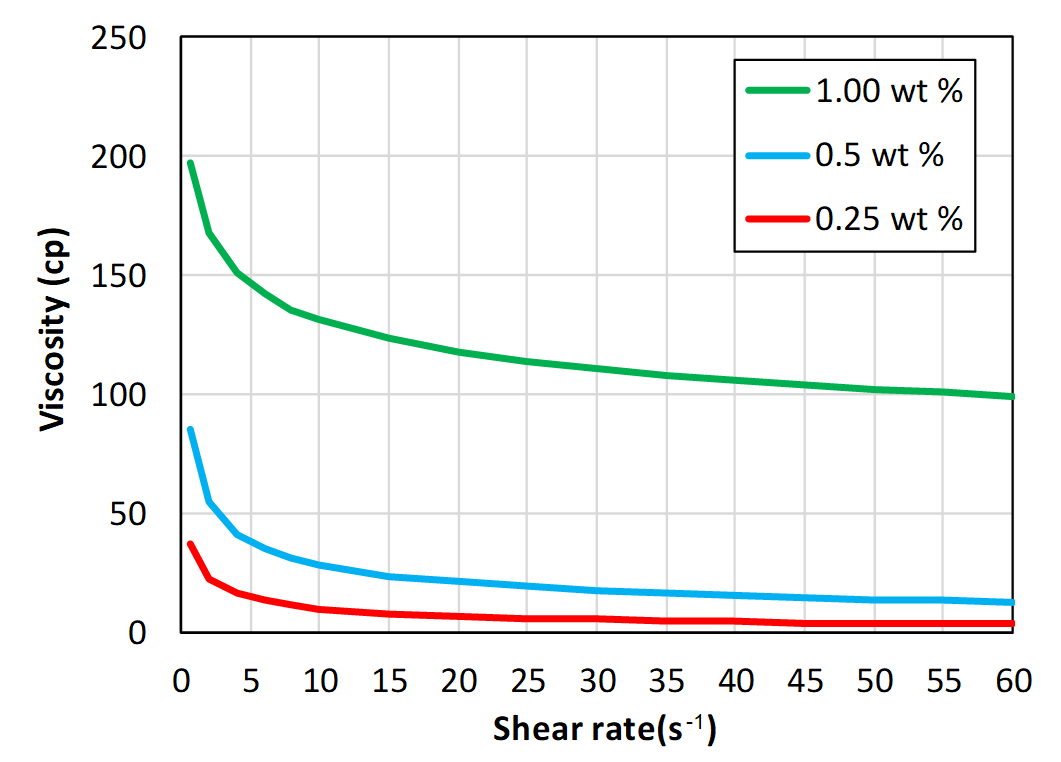
\includegraphics[width=.75\textwidth]{img/cht/viscAlcomer.png}
    \caption{Viscosity as function of shear rate and polymer concentration for Alcomer 24 UK}
    \label{cht:viscAlco}
\end{figure}

\subsubsection{Polyelectrolyte complexes according to the Texas A\&M recipe}

Figure \ref{cht:s10visc50} shows viscosity as function of time on logarithmic and linear scales. As shown in the figure, there were only minor increases in viscosity the first 7 days. After 23 days, the viscosity was increased significantly and it increased further when the last sample was measured after 37 days. Simple power functions were fitted to the experimental data. The plot on linear scale suggest that the largest effect of the cross binding occurred after approximately 20 days. 

\begin{figure}
    \centering
    \makebox[\textwidth][c]{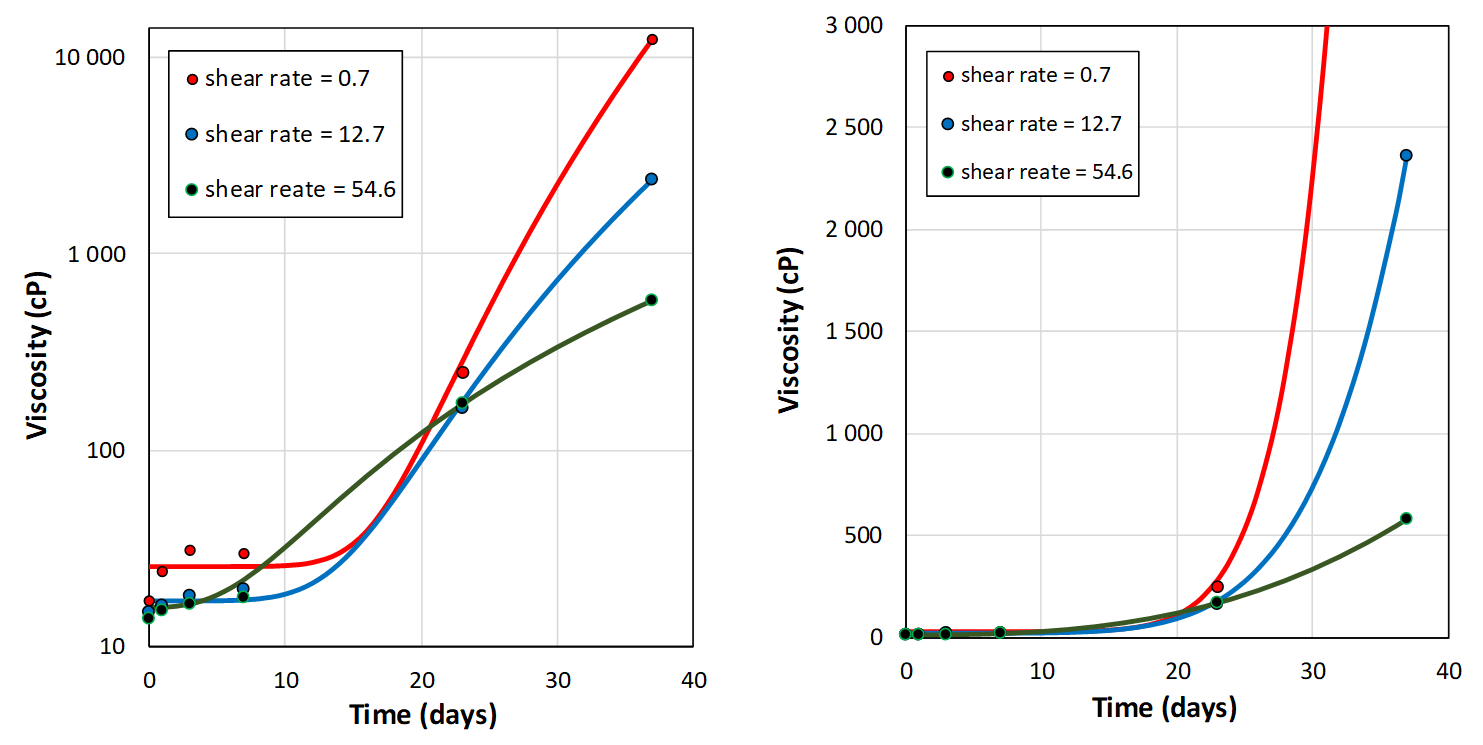
\includegraphics[width=1.2\textwidth]{img/cht/s10visc50.png}}
    \caption{Viscosity as function of aging time for Series 10 samples aged at 50~\celsius~ on logarithmic (left) and linear (right) scales}
    \label{cht:s10visc50}
\end{figure}

Figure \ref{cht:s3536visc} shows the results from viscosity measurements on Series 35 (polymer/PEC solutions made using 0.498 wt. \% of Alcomer 24 UK) and Series 36  0.490 wt. \% of Flopaam 5115 VHM). As seen in Figure \ref{cht:s3536visc}, the viscosity increased quickly, and gels were formed in the vials (visual observations) already after 3 days of aging. The apparent decrease in viscosity at longer aging times are artifacts due to the measurement method as the solutions still appeared as gels.

\begin{figure}
    \centering
    \makebox[\textwidth][c]{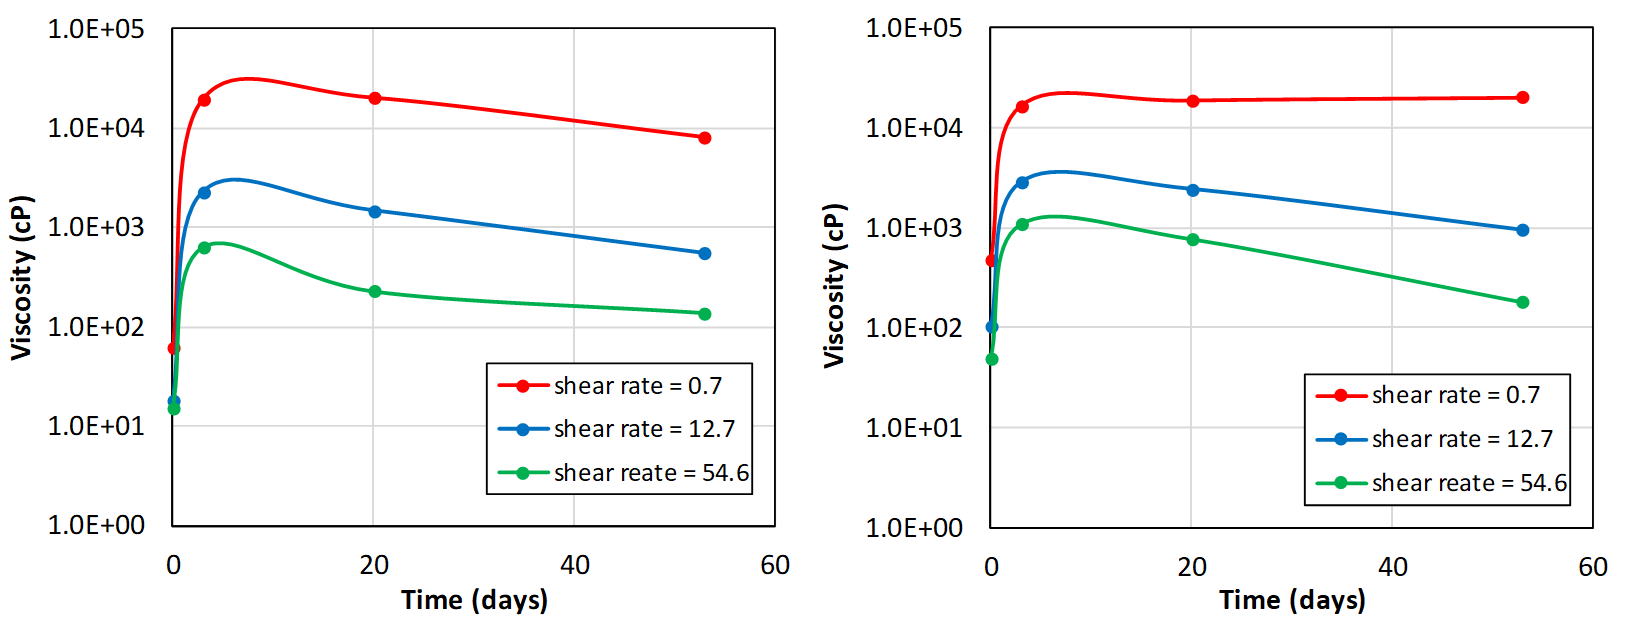
\includegraphics[width=1.2\textwidth]{img/cht/s3536.png}}%
    \caption{Viscosity as function of aging time for Series 35 samples (left) and Series 36 samples (right), aged at 80~\celsius}
    \label{cht:s3536visc}
\end{figure}

Two more systems were made in an equivalent manner using Alcomer 24 UK, but with reduced concentrations of \ce{Cr3+} (60 ppm in Series 42 and 41 ppm in Series 47). Both systems gelled after 3 days of aging at 80~\celsius.


\section{Transport of polymer and nanoparticles through porous media}
\section{ Effect of in-situ gelling on water flow}